\section{Materials \& Methods}
    \subsection{Interviews}
        \subsubsection{Questions}
            \begin{enumerate}
                \item Name? Age? Profession? Level of education?
                \item What mathematics are involved in your day to day life?
                \item What type of calculator is suitable for you?
                \item What functions do you expect a calculator to have?
                \item Would you enjoy having a customizable calculator? Such as different coloured buttons or UI.
                \item Do you prefer having options such as "dark mode", "light mode" or having the option to choose?
                \item Should there be documentation to explain how each function works within the calculator as well as how to interact with the UI?
                \item How accurate do you expect the calculator to be? For example, to the 6th decimal place.
                \item Would you like to be able to keep a history of calculations and their results?
                \item For functions that require you to have several different values for each variable, would you rather they be entered one by one or all at once (in an array)?
                \item Do you want to be able to use the calculator with a command line interface?
                \item Would you like to swap between the pages for the scientific functions and the normal elementary arithmetic functions?
                \item As for the display of the calculator, is it important for you to have a display that can display fractions and symbols as you would write them on paper?
                \item How much would you be willing to pay for this calculator?
                \item Are there any other features that you'd like this calculator to have?
            \end{enumerate}

        \subsubsection{Responses}
            \begin{itemize}
                \item Julies Benson - Car Salesman
                    \begin{enumerate}
                        \item My name is Jules Benson and I am 43 years old. I am a car salesman for Audi. My level of education is a bachelors degree in marketing.
                        \item Normally, I do math when I’m near my desk sitting down with a customer. Math in my job involves calculating the total cost of the vehicle, adding or subtracting vehicle options cost, and more importantly, calculating the monthly payment of the vehicles and the interests.
                        \item The most difficult calculation that I have to do during the whole day is calculating interests that involve a lot of percentages. So for my needs, a basic calculator, without any scientific function is sufficient.
                        \item I expect that a calculator has the ability to do basic calculations obviously. A percentage button would be helpful, that way I wouldn’t have to multiply everything by 100 each time I’m taking a percentage.
                        \item Not necessarily, It wouldn’t change much in my job, I’m looking for practicality over aesthetics.
                        \item My job is during the day, and the dealership is very bright as well, so I don’t really need a dark mode, but I wouldn’t mind it for those winter evenings when the sun goes down early.
                        \item Some documentation would be helpful just to know if there’s some things I previously didn’t know that a calculator can do.
                        \item I expect the calculator to be accurate to the 2nd decimal, which is needed when calculating interests on monthly payments.
                        \item Yes, that would be a good functionality. Sometimes customers are hesitating between different cars and different payment plans, so it will be practical to go back and see the previous calculation for comparison.
                        \item I don’t think I’ll be using that function but if anything, I would want them to be entered one by one.
                        \item I don’t know anything about programming, I am not very tech savvy. So, I don’t want to use it with a command line interface.
                        \item I will most likely be using arithmetic functions, but in some rare case that I end up using scientific functions, it would be a good idea to add a swap between pages just to separate the two functionalities.
                        \item Yes, that would be very helpful, since I wouldn’t have to use my brain too much on plugging in the calculator.
                        \item Around \$20
                        \item I mentioned that a percentage button would be helpful for me, so that’s one thing I would like the calculator to have
                    \end{enumerate}
                \item Chad Smith - Grade 10 Student
                    \begin{enumerate}
                        \item I'm 16 years old, and I'm in grade 10. I don't really have a profession.
                        \item As a high school student, the mathematics which I mostly use is algebra and geometry. But some students including me take advanced math classes which allows me to work on more complex functions like the gamma function.
                        \item I’d like a scientific calculator.
                        \item The calculator should at least have basic arithmetic functions like addition, subtraction, multiplication and division. And along with that it should have some transcendental functions like the logarithmic function, gamma function and arccos(x).
                        \item Yes, having a customizable calculator would allow me to stand out from other students at my school and would make my calculator very unique.
                        \item I would prefer light mode during day-time and dark-mode during nights. So, the option of having both would be the best.
                        \item Yes, a proper user guide explaining all the functions would be helpful.
                        \item I need accuracy to the 4th decimal at least.
                        \item Yes, a recent history of the calculations and their results would be really helpful. Since I’m a student, I work on several problems simultaneously, so going back and checking my previous answers would be really helpful.
                        \item Entering all values at once would be less time consuming and I’d prefer that.
                        \item No, the command line interface for a calculator doesn’t seem necessary to me.
                        \item Swapping between the pages again and again seems very tiring. I’d like it if all the functions are available on the same page.
                        \item I honestly don’t mind either. I’m comfortable with fractions as well as decimals.
                        \item I’m an unemployed 16 year old high school student. So for the calculator we discussed, I could pay max. \$15-\$20
                        \item It’ll be great if the calculator is mobile as well as computer friendly.
                    \end{enumerate}
                \item Shaunna Ross - Sales Representative
                    \begin{enumerate}
                        \item Hello, my name is Shaunna Ross, I am 46 years old. I have a high school degree which has led me to be a sales representative at a retail store.
                        \item At the retail store my daily math consists of simple addition for sales, subtraction for a customer’s return and using percentages to calculate the weekly deals that certain articles of clothing in the store could have. The numbers that come from the computer are crucial to the success of the store, as if those numbers are incorrect, the store can be penalized heavily.
                        \item I just need a simple calculator, not very complicated. I do not need any of the very high math functions that look complicated. Concise is key.
                        \item Well, I definitely think that calculators should always have the basic ones, like adding, subtracting. Even functions I would necessarily use, like multiplication and division are still important to have.I also require the calculator to provide me with 2 decimal places because some clients may pay in cash, and I quickly need to know how much change I may need to give them back. Also as I mentioned before, I need percentages to supply my customers with proper savings and deals.
                        \item It would be interesting to have this functionality. I would love to have this, as I could customize the calculator to fit the theme of my store, and maybe have some customers give their thoughts on an artistic calculator. I could add labels, store icons and colors similar as inside my store.
                        \item I would prefer light mode, as I feel it would be more expressive to how I want my store to run. Although having a dark mode could also be a great addition.
                        \item I personally would like some documentation, as I am not great with computers, and so having documentation could help me a great deal. Also, If I am ever in a hurry, knowing how the buttons work can help me resolve issues that arise.
                        \item I need the calculator to always provide me with 2 decimal places. It is crucial that I provide my customers with exact change if they pay in cash.
                        \item Having a history is extremely important that the calculator has this as a function as I want to be able to provide evidence for customers that what they paid is what they gave me. It is also important to know how much money I have received during the day as I sell more products.Also, it will help me determine If a customer is lying to me for certain transactions. SO yes I would like to keep a history of the calculations.
                        \item I will not really need a functionality for this ever I believe, but if I ever do, I would like to have them one by one.
                        \item To be honest, I do not know what a command line interface is. I am not good with computers, so I would love a simple place where I can press buttons and the actions happen. That tells me that the calculator is working, and that is all I need.
                        \item I do not need a page for scientific functions, even though they could be interesting to use. The basic functions on the front page is perfect for my needs.
                        \item The display should have my number with 2 decimal places. That is perfect for me, since that is what I will use on a daily basis. Fractions are not needed, as I also need to have the customers know how much they are paying. Symbols I would like to have, as they can show me the steps in the purchases or returns of the customers.
                        \item I only need some very easy functions, therefore I am not willing to pay an arm and a leg for a calculator.
                        \item A cool feature that I can request is to have the calculator showcase a simple phrase or couple of words when the calculator is not in use. Adding a “Welcome!” to the calculator will make me buy this product just that much more. The phrase will please customers and illustrate to them that I put a lot of thought into my work environment. This will in turn allow them to trust that they are receiving great clothes.
                    \end{enumerate}
                \item Pierre Cyr - General Contractor
                    \begin{enumerate}
                        \item My name is Pierre Cyr, I am 60 years old. I work as a general contractor for a construction company, and I studied at the Chambre des Notaires du Québec.
                        \item As a general contractor, I use mathematics when working on budgets for construction contracts, which involves finding the quantities required of each material, calculating the total prices for those materials, and how much it will cost for the workers. When on a construction site, I use mathematics to calculate the different distances and areas.
                        \item Something that is simple to use and intuitive. I don’t want to fiddle with a calculator to get the results, I just want it to work. Also not something too small either.
                        \item I expect the “normal” calculator functionalities, plus, minus, multiplication, and division, along with the exponents functions and the trigonometric functions, as I use those quite frequently either when making construction plans or when on the job site, to make sure that the angles are correct.
                        \item I don’t really see the point of customizing the colors of the calculator, as long as the functions are labeled correctly.
                        \item Dark mode is easier on the eyes to use, so I prefer dark mode, but I don’t mind if it is normal.
                        \item As long as the functions are labeled correctly, I don’t think that the documentation on what the button does is necessary, unless the functionality is not intuitive.
                        \item I expect a calculator to have at least 4 decimal positions to get the most accurate result possible, but the more the better. If there aren’t enough then I could get rounding errors, and that would be really bad.
                        \item Keeping a history would help greatly, to check if one of the calculations was incorrect and check on past results.
                        \item I think that in an array would be better, since if I make a mistake entering the results, I can go back to change it, whereas one by one I would have to wait to finish to enter all results before fixing it.
                        \item I would not really have a use for that functionality, no.
                        \item I don’t really have a utility in that, unless the scientific functions really take up a lot of space.
                        \item It would really help if the equations would show up like that, yes. It would be more visually clear if there’s a mistake in the calculation. But how easy would it be to navigate? Because I can move up and down now, it might be a bit difficult to navigate.
                        \item I wouldn’t expect to pay anything just for a calculator, except if it was able to calculate things more easily than using a normal calculator, but even then I wouldn’t spend more than \$5 for it.
                        \item Something that’s always annoyed me with normal calculators is that if there’s a mistake in the calculation, like I forgot to put something after a plus, it waits until I press equal to tell me there was a mistake. Why not let me know beforehand? Also, if you keep track of the history of the calculations, it would be nice to be able to assign a title to the calculation, so that I can remember what it was for. Conversion of units would be quite useful as well, for example to go from sq2 to m2.
                    \end{enumerate}
                \item Jim Turner - Welder
                    \begin{enumerate}
                        \item My name is Jim Turner, age 39, and I graduated high school and then did a DEP in welding.
                        \item As a welder, we use a lot of basic math and some trigonometry in order to cut and weld the right size pieces. The calculator has to be precise, otherwise the final product that we are welding won’t hold the proper shape, and the safety and stability of the structure could be compromised.
                        \item Normally a basic calculator is sufficient enough but we do prefer a scientific calculator since it has the trigonometry functions pre installed.
                        \item As a welder, built in trigonometry functions such as sine, cosine, and tangent would be adequate.
                        \item I would like to have some buttons customized such as a larger equal sign. Buttons should be large so that we have no problems pushing the wrong numbers or functions. I would also like to have a delete button in addition to a clear button so if I make a mistake on one number, I don’t have to clear and start all over. This would help me save time during my work.
                        \item I prefer the option to have both because the lighting in my workplace varies.
                        \item Yes, some basic documentation could be useful.
                        \item As a welder, to the 4th decimal would be ideal. Though less or more would be okay as well.
                        \item Yes, definitely. The history would be very important and it would also be helpful if I can copy/paste the history.
                        \item As a welder, one by one would be best to be able to input each exact custom number and do the steps.
                        \item No, this is not necessary for welders as it will be too time consuming and the average welder does not have that high of computer literacy to use that interface. It’s best to keep it simple.
                       \item Yes, this would be helpful because sometimes we just need basic elementary functions and other times we need the scientific ones. Being able to switch back and forth will make it faster and easier to use when we just need the basic functions.
                        \item No, it’s not because a fraction can mean different values in relation to measurements. It’s easier to just have the numbers and decimals.
                        \item I would be willing to pay up to \$40 if it had all the functions I needed and didn’t drain my device's battery as this is a tool I will be using daily.
                        \item If the calculator is a software/app, it would be a cool feature if we could send a calculation to another user (colleague) so they could see the exact formula and answer. It would also be neat if it had a built-in unit conversion function.
                    \end{enumerate}
                \item Evelyn S. Jones - Security Researcher
                    \begin{enumerate}
                        \item Hello my name is Evelyn S. Jones, I’m 25 years old. I currently work as a Security researcher while I am completing my Masters degree in Information System Security.
                        \item I work with all kinds of math on a daily basis. From basic addition, subtraction, to complex polynomial operations involving both exponential and logarithmic functions. I also use the hexadecimal and binary system often in my work, these are particularly important for me.
                        \item Since my work requires me to switch back and forth between number systems, I would require a fancier calculator than most. A scientific calculator would be able accomplish most of my needs though, having hex and binary conversion would save me a lot of time therefore having a programmer function to allow for that to happen would be great.
                        \item I would expect basic arithmetic functions that allows for at least 9 digits to be shown. At its most basic level it should cover Real Numbers and not deal with imaginary ones. As calculators become more powerful I would expect many more functions that would include polynomials and other statistical functions, like what scientific calculators provide.
                        \item Having a customizable calculator would be pretty cool however I really don’t care too much for having that option. To me a calculator is a tool so having a “pretty” tool just to compute equations isn’t something that really matters to me.
                        \item Personally I prefer dark mode but having the option of both light mode and dark mode is much better. Sometimes I do prefer to switch to light mode because of where my desk is, the light shines on it pretty brightly and I get quite a bit of glare.
                        \item If the calculator has unorthodox functions then yes it should definitely have documentation to explain how they work or how they are laid out. If the calculator has a UI I think it should have documentation since on occasion you get strange layouts that are unintuitive.
                        \item In terms of accuracy I would prefer it to be until the 9th decimal place.
                        \item Having the ability to keep the history of calculations and their results would be great. I often get side tracked and then lose my train of thought so having the history is a great way for me to keep pace on my work in case of sudden distractions.
                        \item As long as I’m made aware of the order of the variables, I would love to have the ability to enter each value in an array format. That way I can double check my values to ensure that they are in fact correct.
                        \item I would prefer for this calculator to have a command line interface. I find that it’s much easier to manually type out the entire equation than to have a pretty GUI.
                        \item I am not a fan of having separate pages for the scientific and basic functions since I use them all in conjunction. If there are many functions then I can understand the need for pages or an “alternative/shift” button that would allow for the use of other functions to compute.
                        \item It is not important for that functionality to be present. However, I can see that if regular people use the calculator they might be more inclined to respond yes to that question. Personally it doesn’t matter to me since programming has made me care less for such functionalities.
                        \item I would not spend anymore than \$50.
                        \item The single feature I would love to have is a decimal to binary/decimal to hex converter that also works vice versa. I go back and forth between these number systems so having them available to me would save me a great amount of time.
                    \end{enumerate}
                \item Ricciardo Rossi - Junior Formula 1 Race Engineer
                    \begin{enumerate}
                        \item Hello, my name is Ricciardo Rossi. I am 38 years old, and I am a junior race engineer for Scuderia Toro Rosso Formula 1 team. I graduated with a master’s degree in software engineering from Sapienza University of Rome. My masters focused mainly on algorithm design with special focus on analysis and optimization.
                        \item I think most people do not realize this, but a race engineer needs to be a jack of all trades that works in liaison with almost all departments including the drivers. Communication needs to be clear and concise to convey important information from the technical department to the driver for them to push the car to the limit. Mathematics is at the center of it all. I do not need to know all the specifics, but I need to have a general idea of what people of various departments are talking about. Therefore, the mathematics involved may be arithmetic, trigonometry, calculus, probability, optimization, and many others. It depends on the day.
                        \item Most of the complicated calculations are already done through the various proprietary software that we use. However, I also have two physical calculators on my desk, just to make sure if one breaks I have a backup. If need be, I use my phone’s calculator for some quick arithmetic if I am on the go.
                        \item A calculator should have general functions such as: basic arithmetic, algebra, logarithms, and trigonometry. In certain situations, the software calculators on my laptop can be an inconvenience to use at certain moments such as when travelling. If the handheld calculator has more key functions such as standard deviation, probability, and calculus, it would be even better.
                        \item I don’t really need any customizable feature in terms of colors for the buttons and UI. However, it would be nice if the customizability extends to complicated functions that general calculators do not have. I guess in that scenario, I would just use a scientific calculator instead haha.
                        \item When I am not having meetings with various departments, I am in front of a screen:  laptops, factory hardware, phones, calculators, and various others. To protect my eyes, I always use them while in dark mode.
                        \item Yes, documentation increases efficiency.
                        \item Honestly, the more accurate the calculator, the better it is for me. Every part of a formula 1 car needs to be designed and made perfectly. Any minute error in our calculations can cost us the race or cause the car to fail. I would therefore expect more than 12 decimal places.
                        \item Yes, that would be a great addition. Keeping history will enable be to backtrack to double check my calculations.
                        \item I see the advantage for both scenarios. I would use the array feature when I have a lot of information to input and vice versa, one by one, when I only have 2 or 3 variables to enter.
                        \item As a race engineer, it would be a great addition to have any calculator. However, most of our complicated calculations are done by our own software, so I would use the command line feature sporadically.
                        \item I believe that would be a great feature to have in order to maintain the logs of your previous calculations.
                        \item It is not important for me.
                        \item I have some flexibility in terms of price. If the calculator gets the job done with no impressive features I am willing to spend \$50. However, if the calculator is able to impress me with its capabilities, I am willing to go up to \$100.
                        \item I would like to be able to export all my calculations and data to files so that I am able to share them with my colleagues.
                    \end{enumerate}
            \end{itemize}

        \subsection{Personas}
            {\raggedright

            \vspace{3pt} \noindent
            \begin{tabular}{|p{130pt}|p{88pt}|p{207pt}|}
            \hline
            \multicolumn{3}{|c|}{\parbox{426pt}{\centering
            Jules Benson
            }} \\
            \hline
            \parbox{130pt}{\raggedright \multirow{6}{*}{
\includegraphics[scale=0.99]{images/julesbenson.png}}} & \parbox{88pt}{\raggedright
            Age:
            } & \parbox{207pt}{\raggedright
            43
            } \\
            \cline{2-3}
             & \parbox{88pt}{\raggedright
            Occupation:
            } & \parbox{207pt}{\raggedright
            Car Salesman
            } \\
            \cline{2-3}
             & \parbox{88pt}{\raggedright
            Skills:
            } & \parbox{207pt}{\raggedright
            \begin{itemize}
                \item Different ways of marketing
                \item Selling products
                \item Influencing people
            \end{itemize}
            } \\
            \cline{2-3}
             & \parbox{88pt}{\raggedright
            Goals:
            } & \parbox{207pt}{\raggedright
            \begin{itemize}
                \item Maximizing vehicle sales
                \item Finding maximum number of new customers everyday.
            \end{itemize}
            } \\
            \cline{2-3}
             & \parbox{88pt}{\raggedright
            Highest Level Of Education:
            } & \parbox{207pt}{\raggedright
            University/Bachelors
            } \\
            \cline{2-3}
             & \parbox{88pt}{\raggedright
            Field Of Study:
            } & \parbox{207pt}{\raggedright
            Marketing
            } \\
            \hline
            \parbox{130pt}{\raggedright
            Background Summary:
            } & \multicolumn{2}{|l|}{\parbox{295pt}{\raggedright
            As a car salesman with a basic understanding of math , Jules seems to be more
            focused on selling to customers rather than doing math.

            Primary use for a calculator would be interest rate calculations for customer
            car payments and calculating vehicle options/add-ons.
            }} \\
            \hline
            \parbox{130pt}{\raggedright
            Desired Functions:
            } & \multicolumn{2}{|l|}{\parbox{295pt}{\raggedright
            Addition, Subtraction, Multiplication, Division
            }} \\
            \hline
            \parbox{130pt}{\raggedright
            Desired Calculator Type:
            } & \multicolumn{2}{|l|}{\parbox{295pt}{\raggedright
            \begin{itemize}
                \item Dark or Light mode calculator
                \item Calculator needs to have at  least  2 decimal accuracy along with a user guide.
                \item A typical GUI.
                \item User guide.
            \end{itemize}
            }} \\
            \hline
            \parbox{130pt}{\raggedright
            Special needs/requirements
            } & \multicolumn{2}{|l|}{\parbox{295pt}{\raggedright
            \begin{itemize}
                \item Needs a percentage button on the calculator.
            \end{itemize}
            }} \\
            \hline
            \parbox{130pt}{\raggedright
            Budget
            } & \multicolumn{2}{|l|}{\parbox{295pt}{\raggedright
            20\$
            }} \\
            \hline
            \end{tabular}
            \vspace{2pt}

            }

            {\raggedright

            \vspace{3pt} \noindent
            \begin{tabular}{|p{130pt}|p{88pt}|p{207pt}|}
            \hline
            \multicolumn{3}{|c|}{\parbox{426pt}{\centering
            Jim Turner
            }} \\
            \hline
            \parbox{130pt}{\raggedright \multirow{6}{*}{
\includegraphics[scale=0.77]{images/jimturner.png}}} & \parbox{88pt}{\raggedright
            Age:
            } & \parbox{207pt}{\raggedright
            28
            } \\
            \cline{2-3}
             & \parbox{88pt}{\raggedright
            Occupation:
            } & \parbox{207pt}{\raggedright
            Welder
            } \\
            \cline{2-3}
             & \parbox{88pt}{\raggedright
            Skills:
            } & \parbox{207pt}{\raggedright
            \begin{itemize}
                \item Stable hands
                \item Manual labor skills
            \end{itemize}
            } \\
            \cline{2-3}
             & \parbox{88pt}{\raggedright
            Goals:
            } & \parbox{207pt}{\raggedright
            \begin{itemize}
                \item Properly cutting shapes
                \item Having precisely welded wood and other products
            \end{itemize}
            } \\
            \cline{2-3}
             & \parbox{88pt}{\raggedright
            Highest Level Of Education:
            } & \parbox{207pt}{\raggedright
            CEGEP/DEP
            } \\
            \cline{2-3}
             & \parbox{88pt}{\raggedright
            Field Of Study:
            } & \parbox{207pt}{\raggedright
            Welding
            } \\
            \hline
            \parbox{130pt}{\raggedright
            Background Summary:
            } & \multicolumn{2}{|l|}{\parbox{295pt}{\raggedright
            Jim Turner is a welder that cares about the perfection of his work. He needs to
            create all sorts of different shapes.

            For this reason, the calculator would be used to calculate the measurements of
            the different types of shapes.
            }} \\
            \hline
            \parbox{130pt}{\raggedright
            Desired Functions:
            } & \multicolumn{2}{|l|}{\parbox{295pt}{\raggedright
            Addition, Subtraction, Multiplication, Division, Trigonometry (sin, cos, tan,
            arcos)
            }} \\
            \hline
            \parbox{130pt}{\raggedright
            Desired Calculator Type:
            } & \multicolumn{2}{|l|}{\parbox{295pt}{\raggedright
            \begin{itemize}
                \item A calculator with both dark and light mode due to workplace settings.
                \item Needs at least 4 decimal accuracy.
                \item A GUI with a large equal sign, clear and delete button.
                \item User guide.
            \end{itemize}
            }} \\
            \hline
            \parbox{130pt}{\raggedright
            Special needs/requirements
            } & \multicolumn{2}{|l|}{\parbox{295pt}{\raggedright
            \begin{itemize}
                \item A ``send'' feature where you can send your equation to a colleague
            \end{itemize}
            }} \\
            \hline
            \parbox{130pt}{\raggedright
            Budget
            } & \multicolumn{2}{|l|}{\parbox{295pt}{\raggedright
            40\$
            }} \\
            \hline
            \end{tabular}
            \vspace{2pt}

            }

            {\raggedright

            \vspace{3pt} \noindent
            \begin{tabular}{|p{130pt}|p{88pt}|p{207pt}|}
            \hline
            \multicolumn{3}{|c|}{\parbox{426pt}{\centering
            Evelyn S. Jones
            }} \\
            \hline
            \parbox{130pt}{\raggedright \multirow{6}{*}{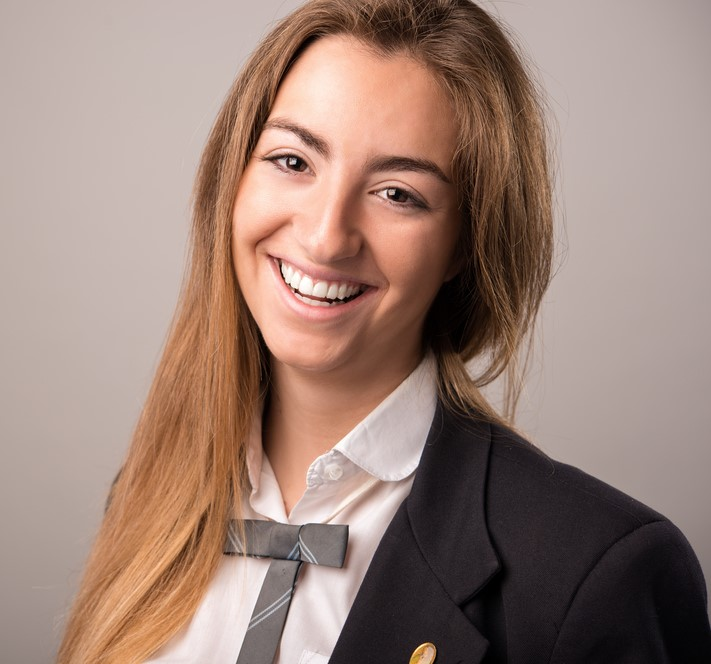
\includegraphics[scale=0.75]{images/evelynsjones.png}}} & \parbox{88pt}{\raggedright
            Age:
            } & \parbox{207pt}{\raggedright
            25
            } \\
            \cline{2-3}
             & \parbox{88pt}{\raggedright
            Occupation:
            } & \parbox{207pt}{\raggedright
            Security Researcher
            } \\
            \cline{2-3}
             & \parbox{88pt}{\raggedright
            Skills:
            } & \parbox{207pt}{\raggedright
            \begin{itemize}
                \item High technology skills
                \item Analytical
            \end{itemize}
            } \\
            \cline{2-3}
             & \parbox{88pt}{\raggedright
            Goals:
            } & \parbox{207pt}{\raggedright
            \begin{itemize}
                \item Accomplishing complex research
                \item Doing difficult mathematics calculator in an easier way
            \end{itemize}
            } \\
            \cline{2-3}
             & \parbox{88pt}{\raggedright
            Highest Level Of Education:
            } & \parbox{207pt}{\raggedright
            University/Masters
            } \\
            \cline{2-3}
             & \parbox{88pt}{\raggedright
            Field Of Study:
            } & \parbox{207pt}{\raggedright
            Information System Security
            } \\
            \hline
            \parbox{130pt}{\raggedright
            Background Summary:
            } & \multicolumn{2}{|l|}{\parbox{295pt}{\raggedright
            Evelyn S. Jones is deeply a very busy person. She is focused on her studies and
            is interning at the same time. She's juggling between 2 roles, both in the same
            field.

            She desires a complex calculator as she's working at a tech job that requires
            complex mathematics. Her research also
            }} \\
            \hline
            \parbox{130pt}{\raggedright
            Desired Functions:
            } & \multicolumn{2}{|l|}{\parbox{295pt}{\raggedright
            Addition, Subtraction, Multiplication, Division, Modulus, Exponential,
            Logarithmic, Floating point, Unit conversion (from decimal to hex or binary and
            vise versa)
            }} \\
            \hline
            \parbox{130pt}{\raggedright
            Desired Calculator Type:
            } & \multicolumn{2}{|l|}{\parbox{295pt}{\raggedright
            \begin{itemize}
                \item A calculator with both dark and light mode.
                \item A calculator with 9 decimal places.
                \item Prefers CLI over a GUI.
                \item User guide/documentation if calculator is unorthodox.
            \end{itemize}
            }} \\
            \hline
            \parbox{130pt}{\raggedright
            Special needs/requirements
            } & \multicolumn{2}{|l|}{\parbox{295pt}{\raggedright
            \begin{itemize}
                \item Decimal to binary/hex conversion and vice-versa
            \end{itemize}
            }} \\
            \hline
            \parbox{130pt}{\raggedright
            Budget
            } & \multicolumn{2}{|l|}{\parbox{295pt}{\raggedright
            $<$=50\$
            }} \\
            \hline
            \end{tabular}
            \vspace{2pt}

            }

            {\raggedright

            \vspace{3pt} \noindent
            \begin{tabular}{|p{140pt}|p{78pt}|p{215pt}|}
            \hline
            \multicolumn{3}{|c|}{\parbox{434pt}{\centering
            Riccardio Rossi
            }} \\
            \hline
            \parbox{140pt}{\raggedright \multirow{6}{*}{
\includegraphics[scale=0.95]{images/riccardiorossi.png}}} & \parbox{78pt}{\raggedright
            Age:
            } & \parbox{215pt}{\raggedright
            38
            } \\
            \cline{2-3}
             & \parbox{78pt}{\raggedright
            Occupation:
            } & \parbox{215pt}{\raggedright
            Junior Race Engineer for Scuderia Toro Rosso F1 team
            } \\
            \cline{2-3}
             & \parbox{78pt}{\raggedright
            Skills:
            } & \parbox{215pt}{\raggedright
            \begin{itemize}
                \item Problem solving, Mathematics
                \item Complex analysis of algorithms
                \item Communication
            \end{itemize}
            } \\
            \cline{2-3}
             & \parbox{78pt}{\raggedright
            Goals:
            } & \parbox{215pt}{\raggedright
            \begin{itemize}
                \item Properly link all the departments in the team
                \item Design and engineering F1 parts that optimize speed to win races without
            compromising safety
            \end{itemize}
            } \\
            \cline{2-3}
             & \parbox{78pt}{\raggedright
            Highest Level Of Education:
            } & \parbox{215pt}{\raggedright
            University/Masters
            } \\
            \cline{2-3}
             & \parbox{78pt}{\raggedright
            Field Of Study:
            } & \parbox{215pt}{\raggedright
            Software Engineering
            } \\
            \hline
            \parbox{140pt}{\raggedright
            Background Summary:
            } & \multicolumn{2}{|l|}{\parbox{294pt}{\raggedright
            Riccardio Rossi is a person that has many responsibilities. On top of acting as
            a liaison between all the departments, his main responsibility is engineering
            different F1 car parts.

            Due to his engineering responsibility, he does advanced mathematical
            calculation. Most of the tools he uses are in his computer but he needs another
            calculator for backup.
            }} \\
            \hline
            \parbox{140pt}{\raggedright
            Desired Functions:
            } & \multicolumn{2}{|l|}{\parbox{294pt}{\raggedright
            Addition, Subtraction, Multiplication, Division, Logarithms, Trigonometry,
            Standard Deviation, Probability and Integrals/Derivatives.
            }} \\
            \hline
            \parbox{140pt}{\raggedright
            Desired Calculator Type:
            } & \multicolumn{2}{|l|}{\parbox{294pt}{\raggedright
            \begin{itemize}
                \item A calculator with dark mode.
                \item Needs max precision: at least 12 decimal points.
                \item Preferably a calculator with both GUI and CLI with history of calculations.
                \item User guide/documentation
            \end{itemize}
            }} \\
            \hline
            \parbox{140pt}{\raggedright
            Special needs/requirements
            } & \multicolumn{2}{|l|}{\parbox{294pt}{\raggedright
            \begin{itemize}
                \item Decimal to binary/hex conversion and vice-versa
            \end{itemize}
            }} \\
            \hline
            \parbox{140pt}{\raggedright
            Budget
            } & \multicolumn{2}{|l|}{\parbox{294pt}{\raggedright
            $<$=50\$
            }} \\
            \hline
            \end{tabular}
            \vspace{2pt}

            }

            {\raggedright

            \vspace{3pt} \noindent
            \begin{tabular}{|p{140pt}|p{78pt}|p{207pt}|}
            \hline
            \multicolumn{3}{|c|}{\parbox{426pt}{\centering
            Chad Smith
            }} \\
            \hline
            \parbox{140pt}{\raggedright \multirow{6}{*}{
\includegraphics[scale=0.98]{images/chadsmith.png}}} & \parbox{78pt}{\raggedright
            Age:
            } & \parbox{207pt}{\raggedright
            16
            } \\
            \cline{2-3}
             & \parbox{78pt}{\raggedright
            Occupation:
            } & \parbox{207pt}{\raggedright
            Student
            } \\
            \cline{2-3}
             & \parbox{78pt}{\raggedright
            Skills:
            } & \parbox{207pt}{\raggedright
            \begin{itemize}
                \item Problem solving
                \item Critical thinking
                \item Advanced math
            \end{itemize}
            } \\
            \cline{2-3}
             & \parbox{78pt}{\raggedright
            Goals:
            } & \parbox{207pt}{\raggedright
            \begin{itemize}
                \item Basic math calculations for algebra and geometry
                \item Using complex math functions for advanced math classes
            \end{itemize}
            } \\
            \cline{2-3}
             & \parbox{78pt}{\raggedright
            Highest Level Of Education:
            } & \parbox{207pt}{\raggedright
            10th grade in High School
            } \\
            \cline{2-3}
             & \parbox{78pt}{\raggedright
            Field Of Study:
            } & \parbox{207pt}{\raggedright
            N/A
            } \\
            \hline
            \parbox{140pt}{\raggedright
            Background Summary:
            } & \multicolumn{2}{|l|}{\parbox{285pt}{\raggedright
            Chad Smith is a 16 year old high school student. As a high school student, he
            needs a normal calculator for his Math, Physics and Chemistry classes. But along
            with these, he's taking Advanced Math classes which allows him to work on complex
            math functions like the gamma function. He would like a calculator with an
            easy-to-use user interface and saved history.
            }} \\
            \hline
            \parbox{140pt}{\raggedright
            Desired Functions:
            } & \multicolumn{2}{|l|}{\parbox{285pt}{\raggedright
            Basic arithmetic functions, Logarithmic function, Gamma function and arccos(x),
            sinh(x), ab\textasciicircum{}x, Standard Deviation and Mean Absolute Deviation.
            }} \\
            \hline
            \parbox{140pt}{\raggedright
            Desired Calculator Type:
            } & \multicolumn{2}{|l|}{\parbox{285pt}{\raggedright
            \begin{itemize}
                \item A calculator with both dark and light mode.
                \item Needs precision of at least 4 decimal points.
                \item Prefers GUI over a CLI.
                \item User guide/documentation
            \end{itemize}
            }} \\
            \hline
            \parbox{140pt}{\raggedright
            Special needs/requirements
            } & \multicolumn{2}{|l|}{\parbox{285pt}{\raggedright
            \begin{itemize}
                \item Make it mobile and computer friendly
            \end{itemize}
            }} \\
            \hline
            \parbox{140pt}{\raggedright
            Budget
            } & \multicolumn{2}{|l|}{\parbox{285pt}{\raggedright
            \$15 - \$20
            }} \\
            \hline
            \end{tabular}
            \vspace{2pt}

            }

            {\raggedright

            \vspace{3pt} \noindent
            \begin{tabular}{|p{140pt}|p{78pt}|p{207pt}|}
            \hline
            \multicolumn{3}{|c|}{\parbox{426pt}{\centering
            Shaunna Ross
            }} \\
            \hline
            \parbox{140pt}{\raggedright \multirow{6}{*}{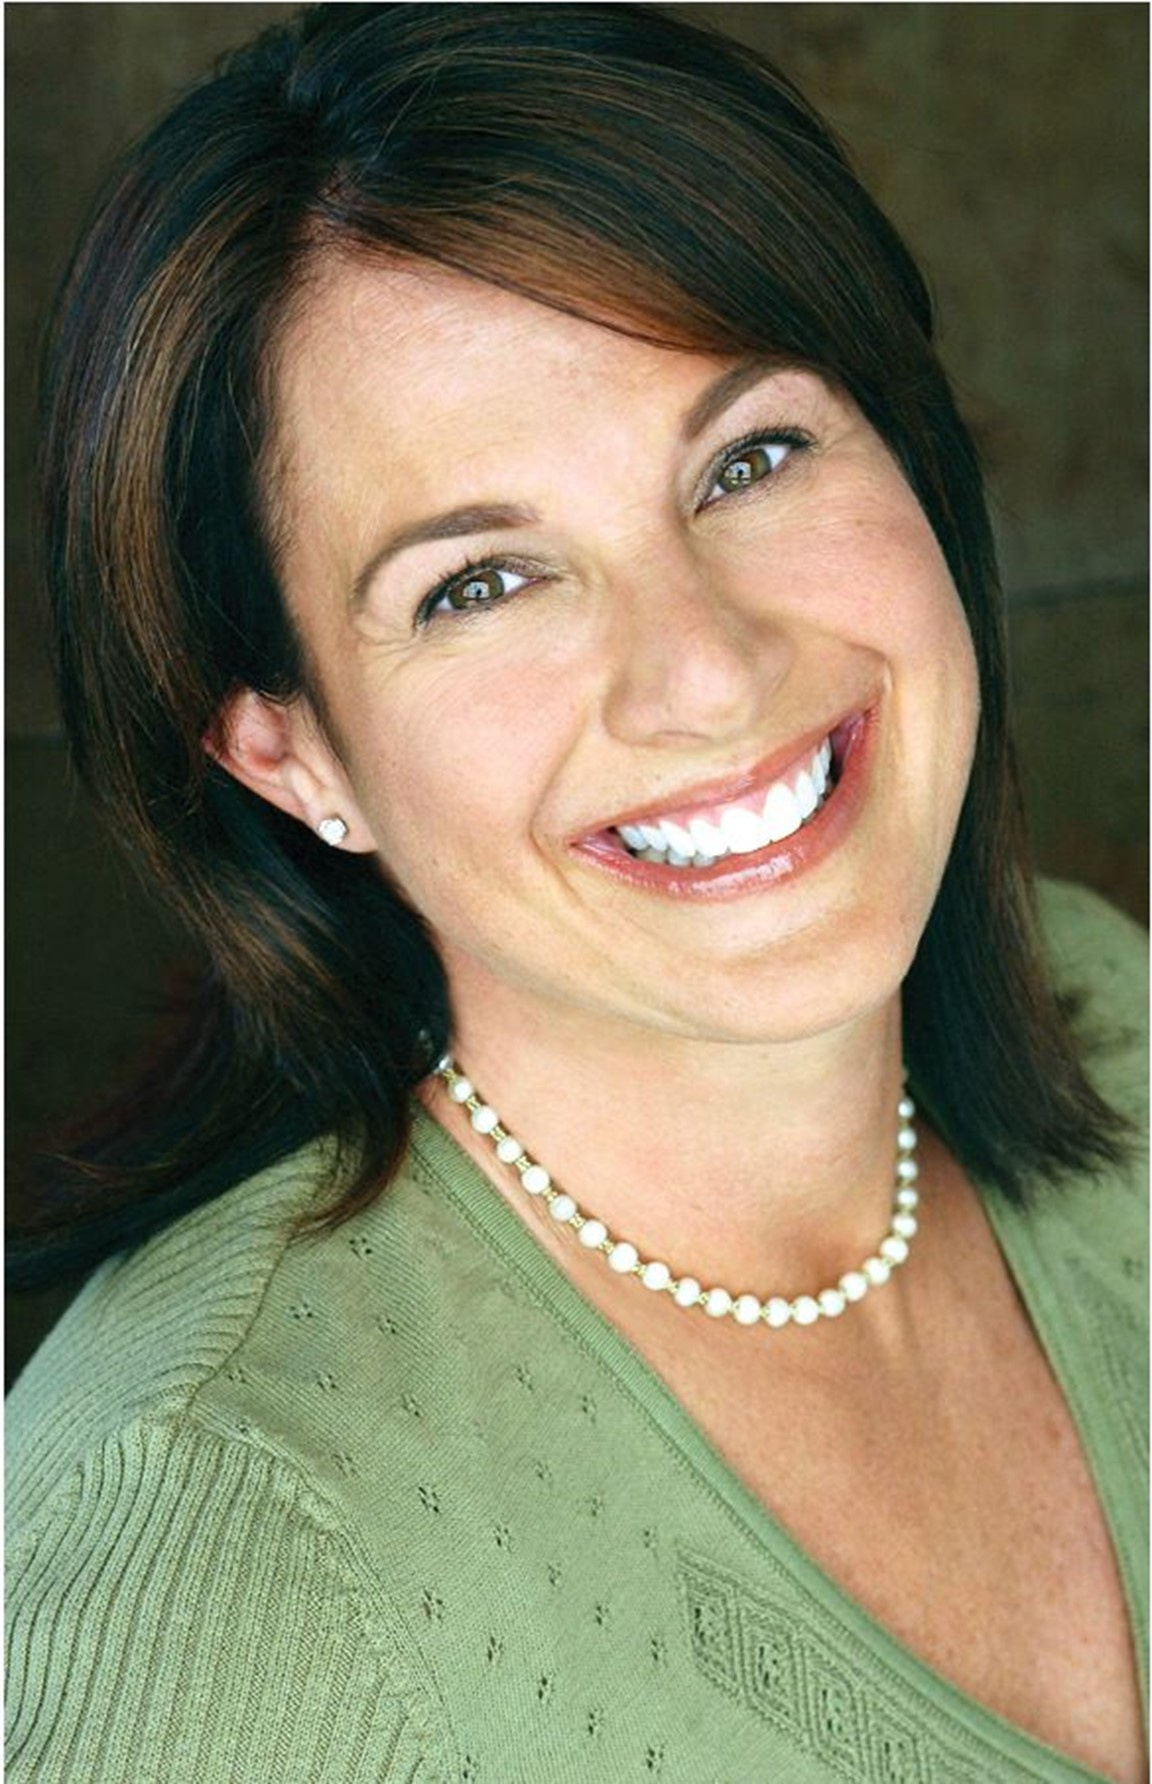
\includegraphics[scale=0.87]{images/shaunnaross.png}}} & \parbox{78pt}{\raggedright
            Age:
            } & \parbox{207pt}{\raggedright
            46
            } \\
            \cline{2-3}
             & \parbox{78pt}{\raggedright
            Occupation:
            } & \parbox{207pt}{\raggedright
            Sales Representative
            } \\
            \cline{2-3}
             & \parbox{78pt}{\raggedright
            Skills:
            } & \parbox{207pt}{\raggedright
            \begin{itemize}
                \item Communication skills
                \item Sales
                \item Customer service
            \end{itemize}
            } \\
            \cline{2-3}
             & \parbox{78pt}{\raggedright
            Goals:
            } & \parbox{207pt}{\raggedright
            \begin{itemize}
                \item Using addition for sales
                \item Using subtraction for customer's return
                \item Using percentages to calculate weekly deals
            \end{itemize}
            } \\
            \cline{2-3}
             & \parbox{78pt}{\raggedright
            Highest Level Of Education:
            } & \parbox{207pt}{\raggedright
            High School Diploma
            } \\
            \cline{2-3}
             & \parbox{78pt}{\raggedright
            Field Of Study:
            } & \parbox{207pt}{\raggedright
            N/A
            } \\
            \hline
            \parbox{140pt}{\raggedright
            Background Summary:
            } & \multicolumn{2}{|l|}{\parbox{285pt}{\raggedright
            Shaunna Ross is a 46 year old sales representative who deeply cares about her
            customers. She uses a calculator at her retail store for her daily math
            calculations which includes basic math functions like addition, subtraction and
            percentages. She thinks that the numbers that come from the calculator are
            crucial to the success of the store, as if those numbers are incorrect, the store
            can be heavily penalised.
            }} \\
            \hline
            \parbox{140pt}{\raggedright
            Desired Functions:
            } & \multicolumn{2}{|l|}{\parbox{285pt}{\raggedright
            Addition, Subtraction, Multiplication, Division and Percent.
            }} \\
            \hline
            \parbox{140pt}{\raggedright
            Desired Calculator Type:
            } & \multicolumn{2}{|l|}{\parbox{285pt}{\raggedright
            \begin{itemize}
                \item A calculator with light mode.
                \item Needs precision of at least 2 decimal points.
                \item Prefers GUI over a CLI.
                \item User guide/documentation
            \end{itemize}
            }} \\
            \hline
            \parbox{140pt}{\raggedright
            Special needs/requirements
            } & \multicolumn{2}{|l|}{\parbox{285pt}{\raggedright
            \begin{itemize}
                \item Percentage button in the calculator
            \end{itemize}
            }} \\
            \hline
            \parbox{140pt}{\raggedright
            Budget
            } & \multicolumn{2}{|l|}{\parbox{285pt}{\raggedright
            \$5 - \$10
            }} \\
            \hline
            \end{tabular}
            \vspace{2pt}

            }

            {\raggedright

            \vspace{3pt} \noindent
            \begin{tabular}{|p{140pt}|p{78pt}|p{207pt}|}
            \hline
            \multicolumn{3}{|c|}{\parbox{426pt}{\centering
            Pierre Cyr
            }} \\
            \hline
            \parbox{140pt}{\raggedright \multirow{6}{*}{
\includegraphics[scale=1.1]{images/pierrecyr.png}}} & \parbox{78pt}{\raggedright
            Age:
            } & \parbox{207pt}{\raggedright
            60
            } \\
            \cline{2-3}
             & \parbox{78pt}{\raggedright
            Occupation:
            } & \parbox{207pt}{\raggedright
            General Contractor
            } \\
            \cline{2-3}
             & \parbox{78pt}{\raggedright
            Skills:
            } & \parbox{207pt}{\raggedright
            \begin{itemize}
                \item Attention to detail
                \item Responsible
                \item Leadership skills
            \end{itemize}
            } \\
            \cline{2-3}
             & \parbox{78pt}{\raggedright
            Goals:
            } & \parbox{207pt}{\raggedright
            \begin{itemize}
                \item Budgeting for construction contracts
                \item Calculating different distances and areas
                \item Basic math calculations
            \end{itemize}
            } \\
            \cline{2-3}
             & \parbox{78pt}{\raggedright
            Highest Level Of Education:
            } & \parbox{207pt}{\raggedright
            Studied at the Chambre des Notaires du Qu\'{e}bec
            } \\
            \cline{2-3}
             & \parbox{78pt}{\raggedright
            Field Of Study:
            } & \parbox{207pt}{\raggedright
            N/A
            } \\
            \hline
            \parbox{140pt}{\raggedright
            Background Summary:
            } & \multicolumn{2}{|l|}{\parbox{285pt}{\raggedright
            Pierre Cyr is a 60 year old general contractor at a construction company. His
            job requires very high attention to detail and would therefore like a calculator
            with at least 4 decimal positions to get the most accurate result.
            }} \\
            \hline
            \parbox{140pt}{\raggedright
            Desired Functions:
            } & \multicolumn{2}{|l|}{\parbox{285pt}{\raggedright
            Basic math functions and trigonometric functions
            }} \\
            \hline
            \parbox{140pt}{\raggedright
            Desired Calculator Type:
            } & \multicolumn{2}{|l|}{\parbox{285pt}{\raggedright
            \begin{itemize}
                \item A calculator with dark mode.
                \item Needs precision of at least 4 decimal points.
                \item Prefers GUI over a CLI.
                \item User guide/documentation is not necessary
            \end{itemize}
            }} \\
            \hline
            \parbox{140pt}{\raggedright
            Special needs/requirements
            } & \multicolumn{2}{|l|}{\parbox{285pt}{\raggedright
            \begin{itemize}
                \item Indication that the calculation is incorrect before pressing equal
            \end{itemize}
            }} \\
            \hline
            \parbox{140pt}{\raggedright
            Budget
            } & \multicolumn{2}{|l|}{\parbox{285pt}{\raggedright
            Free - \$5
            }} \\
            \hline
            \end{tabular}
            \vspace{2pt}

            }


            \FloatBarrier

        \newpage
        \subsection{Use Cases}
            \begin{figure}[!htb]
                \centering
                \includegraphics[scale=0.5]{images/usecases.PNG}
            \end{figure}
            \paragraph{}
            In the figure above, we illustrate all possible use cases for our product. To demonstrate several examples, consider the following:
            \begin{itemize}
                \item Use case \#1: Launch ETERNITY -$>$ Enters expression: y = 2(3) + 5 -$>$ ETERNITY parses expression -$>$ Interpreter handles calculation -$>$ Simple Arithmetic -$>$ Returns answer: 11 -$>$ Clears screen -$>$ Closes ETERNITY
                \item Use case \#2: Launch ETERNITY -$>$ Enters expression: 1 + 2 -$>$ ETERNITY parses expression -$>$ Interpreter handles calculation -$>$ Simple Arithmetic -$>$ Returns answer: 3 -$>$ Clears screen -$>$ Enters expression: 3 * 4 -$>$ ETERNITY parses expression -$>$ Interpreter handles calculation -$>$ Simple Arithmetic -$>$ Returns answer: 12 -$>$ Check history -$>$ Select previous equation (1 + 2) -$>$ Modify expression: 2 + 4 -$>$ ETERNITY parses expression -$>$ Interpreter handles calculation -$>$ Simple Arithmetic -$>$ Returns answer: 6 -$>$ Clears screen -$>$ Closes ETERNITY
                \item Use case \#3: Launch ETERNITY -$>$ Customizes UI -$>$ Change to dark mode -$>$ Enter expression: arccos(.5) -$>$ ETERNITY parses expression -$>$ Interpreter handles calculation -$>$ Complex Arithmetic -$>$ Returns answer: 1.047197551 RAD
                \item Use case \#4: Launch ETERNITY -$>$ Enters expression: 10 / 2 -$>$ ETERNITY parses expression -$>$ Interpreter handles calculation -$>$ Simple Arithmetic -$>$ Returns 2 -$>$ Clears screen -$>$ Check history -$>$ Clear history -$>$ Closes ETERNITY
            \end{itemize}
            \FloatBarrier
